%\section{Properties of data passing the preselection}
%\label{sec:bulk}

Figure~\ref{fig:bulk} compares several kinematic distributions in data and SM MC for events passing the preselection.
As an illustration, we also show the MC distributions for the LM1 benchmark point. We find that the SM MC reproduces 
the properties of the bulk of dilepton $t\bar{t}$ events. 
%We therefore turn our attention to the tails of the \MET\ and \HT\ 
%distributions of the $t\bar{t}$ sample. 


\begin{figure}[tbh]
\begin{center}
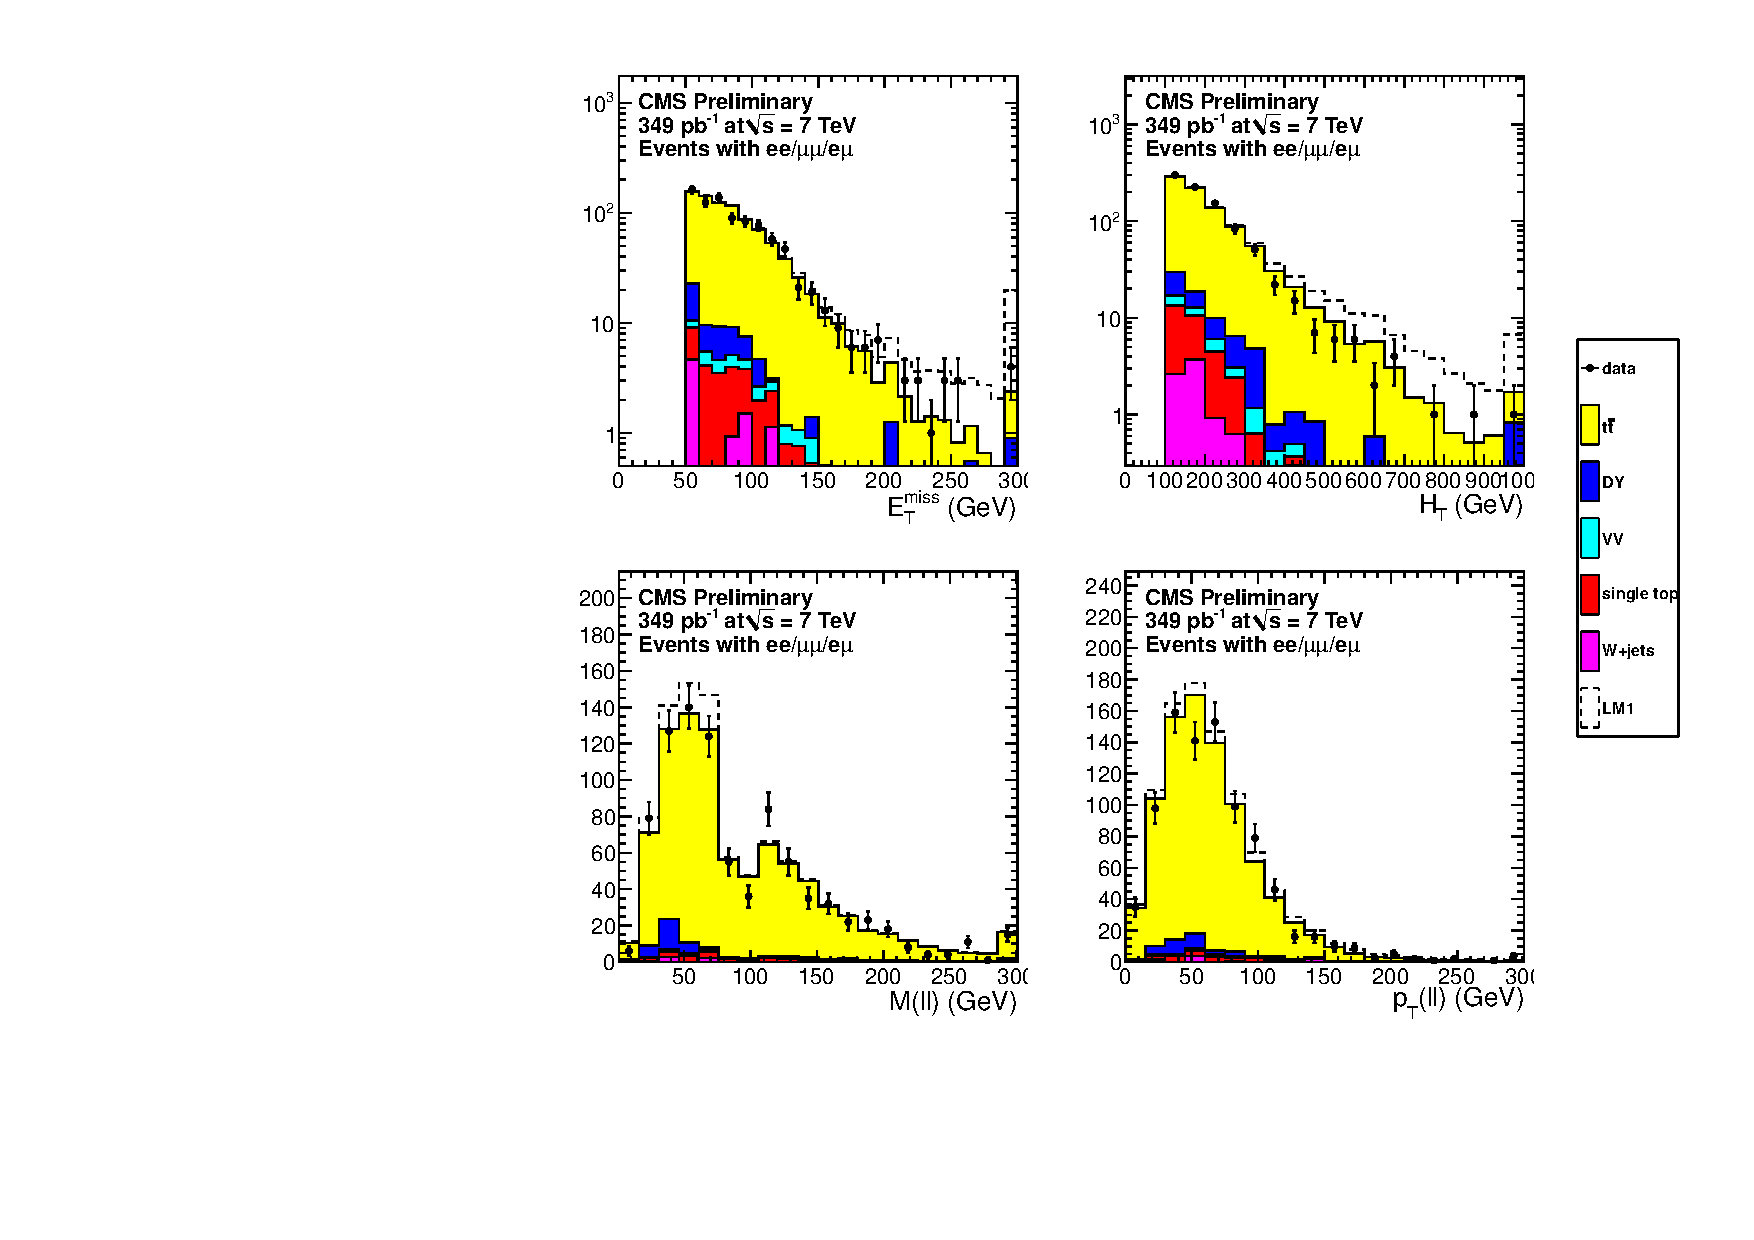
\includegraphics[width=1.0\linewidth]{plots_final/datamc_LM1_349pb.pdf}
\caption{\label{fig:bulk}\protect 
Distributions of (top left) missing tranverse energy \MET, (top right) scalar sum of jet transverse energies (\HT), 
(bottom left) dilepton invariant mass $M(\ell\ell)$, and (bottom right) dilepton transverse momentum $\pt(\ell\ell)$ 
for SM MC and data after preselection. The last bin contains the overflow.
The MC has been normalized to match the data by applying a scale factor of 1.12.
Here $VV$ indicates the sum of $WW$, $WZ$, and $ZZ$. 
The MC distributions for the LM1 benchmark point are also shown.
}
\end{center}
\end{figure}
